% Quickly landscape for experiment page.
\newcommand{\landscapeexperimentpage}[1]{{
\begin{landscape}
  \begin{minipage}[t]{0.97\linewidth}
    \raggedleft
    \begin{minipage}[t]{0.97\linewidth}
      \centering
      #1
    \end{minipage}
  \end{minipage}
\end{landscape}
}}

% Quickly create the table.
\newcommand{\gasettingstable}[4]{{
\begin{table}[H]
  \centering
  \caption{實驗 #2 之基因演算法參數配置}
  \label{tbl:settings-of-experiment-#1}
  \bigskip
  \vspace{-5mm}
  \begin{minipage}[t]{0.35\linewidth}
    \centering
    \begin{tabular}[t]{| c | c | c |}
      \hline
      \multicolumn{1}{ |c| }{回合次數}
        & \multicolumn{1}{ c| }{世代數量}
        & \multicolumn{1}{ c| }{個體數量} \\\hline
      #3
      \hline
    \end{tabular}
  \end{minipage}
  \begin{minipage}[t]{0.35\linewidth}
    \centering
    \begin{tabular}[t]{| c | c | c |}
      \hline
      \multicolumn{1}{ |c| }{指標}
        & \multicolumn{1}{ c| }{權重}
        & \multicolumn{1}{ c| }{備注} \\\hline
      #4
      \hline
    \end{tabular}
  \end{minipage}
\end{table}
}}

% Quickly show the evolution results via figure.
\newcommand{\galayoutresults}[2]{{
\includegraphics[width=0.90\linewidth]{figures/experiments/#1-results.pdf}
\captionof{figure}{實驗 #2 的演化結果及各演化耗時}
\label{fig:experiment-#1-results}
}}

% Quickly create the table.
\newcommand{\garesultssubtable}[1]{{
\begin{minipage}[t]{0.48\linewidth}
  \centering
  \begin{tabular}[t]{
    | >{\centering\arraybackslash}m{0.8cm}
    | >{\centering\arraybackslash}m{1.7cm}
    | >{\centering\arraybackslash}m{1.5cm} 
    | >{\centering\arraybackslash}m{1.0cm} | }
    \hline
    \multirow{2}{*}{回合} & 指標 & \multicolumn{1}{ c| }{適應值} & \multicolumn{1}{ c| }{權重} \\\cline{2-4}
    & \multicolumn{3}{ c| }{總適應值} \\\hline
    #1
  \end{tabular}
\end{minipage}
}}

\newcommand{\garesultstable}[5]{{
\begin{table}[H]
  \centering
  \caption{實驗 #2 - 共 #3 回合的最佳個體之標準化加權適應值}
  \label{tbl:result-of-experiment-#1}
  \bigskip
  \vspace{-5mm}
  \garesultssubtable{#4}
  \garesultssubtable{#5}
\end{table}
}}

\chapter{實驗結果與分析}
\label{cha:experiment}

本章節將探討前述章節之方法是否符合研究目標:第~\ref{sec:experiment-definition} 節,對本次實驗之環境建置、演算法使用之參數進行解釋;第~\ref{sec:experiment-diagram} 節
,描述本次研究實驗之各項步驟;第~\ref{sec:experiment-results} 節,針對所挑選的房間採用不同權重的適應性函數,其族群大小會如何影響房間內的遊戲物件之佈局結果。

\section{實驗定義}
\label{sec:experiment-definition}

我們使用 Invector 公司開發的 \textit{Third Person Controller - Melee Combat Template} 套件(以下簡稱 \textit{3rdPC})進行遊戲物件的設置。\textit{3rdPC} 提供遊戲開發者快速建構玩家控制角色 (Player Character) 、非玩家控制角色 (Non-Player Character) 與其角色控制器或人工智能,並可製作任何類型的第三人稱動作冒險遊戲或角色扮演遊戲。第~\ref{ssec:experiment-gameplaymanual} 小節中,說明 \textit{3rdPC} 提供的玩家角色的操作使用說明;第~\ref{ssec:experiment-gameobjects} 小節中,解釋實驗中的採用遊戲物件,其象徵意義與玩家角色互動方式;第~\ref{ssec:experiment-parameters} 小節中,將定義屬實驗變因的相關參數設定,包含任務語法與基因演算法。

\subsection{遊戲操作說明}
\label{ssec:experiment-gameplaymanual}

玩家所控制的角色能夠移動、攻擊、防禦、跳躍與蹲下等動作。移動使用方向鍵,角色朝前後左右與其斜向組合鍵的方向移動,過程中按下 shift 按鍵將會切換至奔跑模式;攻擊使用滑鼠左鍵單擊,連續使用能夠進行三階段的攻擊,每次攻擊將消耗耐力值;防禦使用滑鼠右鍵單擊,能夠減少受到敵方攻擊的損傷;跳躍按鍵鍵盤 space 按鍵,角色能夠進行原地跳躍,在移動或奔跑的過程中亦可使用;蹲下按下鍵盤 c 按鍵,角色能夠緩慢的移動,適合觀察敵方戰況的同時進行移動。

\subsection{遊戲物件說明}
\label{ssec:experiment-gameobjects}

敵人會在玩家靠近,且進入攻擊視野範圍時,追擊玩家。當玩家靠近並朝向寶箱時,按下鍵盤 E 按鍵便可以開啟寶箱,取得寶箱內容物。當玩家碰觸到陷阱時,會受到一定程度的損傷。

% \subsubsection{敵人}
% \label{sssec:experiment-gameobjects-enemy}

% 敵人 (編輯中)。

% \subsubsection{寶箱}
% \label{sssec:experiment-gameobjects-treasure}

% 當玩家靠近並朝向寶箱時,按下鍵盤 E 按鍵便可以開啟寶箱,取得寶箱內容物。

% \subsubsection{陷阱}
% \label{sssec:experiment-gameobjects-trap}

% 當玩家碰觸到陷阱時,會受到一定程度的損傷。

\subsection{實驗參數設定與名詞解釋}
\label{ssec:experiment-parameters}

本次實驗中將專注於檢視遊戲物件佈局的結果,而任務語法將沿用圖~\ref{fig:mission-to-space-instruction-flow} 所生成之任務圖,為使實驗結果清晰易讀,將移除無關聯之房間容器於實驗範例。房間容器的遊戲物件佈局演化階段時,每一次世代的演化過程有 $80\%$ 機率於父母代進行兩點交配 (two-point crossover);$10\%$ 機率令衍生子代會進行突變,個體的染色體有 $5\%$ 至 $20\%$ 的基因會轉換成其它的遊戲物件種類,設定值參考自~\cite{liapis2017multi}。相關實驗所使用之名詞,請參照表~\ref{tbl:definition-of-terms-in-experiment} 之釋義。

然而各個房間容器的適應性函數之權重如何決定?將取決於關卡設計師對於該房間容器預期產出進行調整,若希望該遊玩特徵指標能愈出現於房間容器,則將其權重調高 $w = (0, 1]$;反之,愈不希望該遊玩特徵指標出現在房間容器,則將其權重調低 $w = [-1, 0)$;若不理會該遊玩特徵指標的體現與否,則將其權重設定為 $w = 0$。在本次研究的系列實驗中,將以關卡設計師視角進行權重的指派,並不代表實驗中所使用的權重最能夠體現其房間容器。

\setlength\LTcapwidth{\linewidth}
\begin{longtable}{
    | >{\arraybackslash} m{4.0cm}
    | >{\arraybackslash} m{8.5cm} | }
  \caption{實驗使用之名詞釋義}\label{tbl:definition-of-terms-in-experiment} \\
  \hline
  \multicolumn{1}{ |c| }{名詞} & \multicolumn{1}{ c| }{名詞解釋} \\
  \hline
  \endfirsthead
  \multicolumn{2}{c}%
  {\tablename\ \thetable\ -- \textit{接續前頁面}} \\
  \hline
  \multicolumn{1}{ |c| }{名詞} & \multicolumn{1}{ c| }{名詞解釋} \\
  \hline
  \endhead
  \multicolumn{2}{r}{\textit{接續下頁面}} \\
  \endfoot
  \endlastfoot
  回合 (run)
    & 回合為使用相同參數進行的實驗,但實驗間的演化過程與結果是彼此獨立進行。 \\\hline
  世代 (generation)
    & 世代為完整地完成一輪的演化,包含了擇優交配、子代突變與世代交替。 \\\hline
  族群 (population)
    & 族群為每世代中個體的數量。 \\\hline
  個體 (individual)
    & 個體為染色體集合的單位,在本次實驗環境中個體僅有一條染色體,該染色體為遊戲物件佈局的基因序列。 \\\hline
  相鄰
    & 周圍是特定一遊戲物件,其相距僅一格正四方或一格斜四方的距離範圍內的其它遊戲物件。 \\\hline
  標準化加權適應值
    & 原始的適應值進行標準化處理後,並依照對應權重值進行加權,最後得到一數值 $score = [-1, 1]$。 \\\hline
\end{longtable}

\section{實驗流程}
\label{sec:experiment-diagram}

\subsection{透過任務語法建立任務圖}
\label{ssec:experiment-diagram-missiongrammars}

第一步驟,藉由第~\ref{sec:method-missiongrammars} 節所介紹的任務語法與改寫系統 I,搭配任務符號表(表~\ref{tbl:mission-grammars-alphabet-default}、~\ref{tbl:mission-grammars-alphabet})以及任務規則表(表~\ref{tbl:missiongrammars-rules-linear-example}、~\ref{tbl:missiongrammars-rules-nonlinear-example1}、~\ref{tbl:missiongrammars-rules-nonlinear-example2}、~\ref{tbl:missiongrammars-rules-nonlinear-example3}),進行任務圖的生成工作。




\subsection{基於任務圖轉換為遊戲空間}
\label{ssec:experiment-diagram-missiontospace}

第二步驟,基於前一小節所生成的任務圖(圖XXXXXXXXXXXXXXXXXXXXXXXXXXXXXX),搭配第~\ref{sec:method-spacepieces} 節所建置的房間容器(圖~\ref{fig:roomtype-mainpath-i}、~\ref{fig:roomtype-mainpath-ii}、~\ref{fig:roomtype-special}、~\ref{fig:roomtype-wall}),與其對應的建造方式表(表~\ref{tbl:mission-to-space-instruction})與空間替換表(表~\ref{tbl:mission-to-space-replace}),將該任務圖轉換為遊戲空間。




\subsection{資料收集}
\label{ssec:experiment-diagram-datacollection}

第三步驟,將收集第~\ref{sec:method-segments} 節中,房間容器進行基因演算法演化時,於演化過程中收集下述資訊並輸出 CSV 格式資料:

\begin{itemize}
  \vspace{-5mm}
  \setlength\itemsep{-0.5em}
  \item 紀錄各回合、世代中,其各個個體(單一染色體)的適應值經標準化後的得分狀況,見表~\ref{tbl:structure-of-rawdata-scores}。
  \item 紀錄各回合、世代中,其各個個體(單一染色體)的所有座標資訊與其遊戲物件類型,見表~\ref{tbl:structure-of-rawdata-positions}。
  \item 在每一回合結束時,會輸出其演化運算之耗時。更多的原始資料節錄內容可參見附錄資源。
\end{itemize}

\begin{table}[!htb]
  \centering
  \caption{演化適應值資料節錄示意}
  \label{tbl:structure-of-rawdata-scores}
  \bigskip
  \vspace{-5mm}
  \begin{tabular}{| c | c | c | c | r |}
    \hline
    \multicolumn{1}{ |c| }{回合編號}
      & \multicolumn{1}{ c| }{世代編號}
      & \multicolumn{1}{ c| }{個體編號}
      & \multicolumn{1}{ c| }{指標}
      & \multicolumn{1}{ c| }{標準化加權適應值} \\\hline
    $1$ & $1$ & $1$ & 阻擋點       & $0$ \\
    $1$ & $1$ & $1$ & 巡邏點       & $0$ \\
    $1$ & $1$ & $1$ & 守衛點       & $0$ \\
    $1$ & $1$ & $1$ & 遊戲物件數量 & $0$ \\
    $1$ & $1$ & $2$ & 阻擋點       & $0.6540$ \\
    $1$ & $1$ & $2$ & 巡邏點       & $0.5587$ \\
    \hline
  \end{tabular}
\end{table}

\begin{table}[!htb]
  \centering
  \caption{演化座標資料節錄示意}
  \label{tbl:structure-of-rawdata-positions}
  \bigskip
  \vspace{-5mm}
  \begin{tabular}{| c | c | c | l | c |}
    \hline
    \multicolumn{1}{ |c| }{回合編號}
      & \multicolumn{1}{ c| }{世代編號}
      & \multicolumn{1}{ c| }{個體編號}
      & \multicolumn{1}{ c| }{座標}
      & \multicolumn{1}{ c| }{遊戲物件類型} \\\hline
    $1$ & $1$ & $1$ & $(1.0, 1.0, 0.0)$ & $Treasure$ \\
    $1$ & $1$ & $1$ & $(0.0, 1.0, 0.0)$ & $Empty$ \\
    $1$ & $1$ & $1$ & $(0.0, 1.0, 2.0)$ & $Empty$ \\
    $1$ & $1$ & $2$ & $(1.0, 1.0, 0.0)$ & $Enemy$ \\
    $1$ & $1$ & $2$ & $(0.0, 1.0, 0.0)$ & $Empty$ \\
    \hline
  \end{tabular}
\end{table}

\subsection{房間容器演化}
\label{ssec:experiment-diagram-volumesevolution}



\section{房間容器佈局演化之結果}
\label{sec:experiment-results}

在第~\ref{ssec:method-segments-appliedonvolumes} 小節中,展示了寶藏房與戰鬥通道(狹路驅逐、鎮守要道)三種空間的局部佈局演化結果,隨著房間容器搭配不同的適應性函數,便能夠生成出多樣性的遊戲物件佈局。在本小節的各實驗中,將針對上述三種房間容器的演化結果做更進一步的分析,紀錄佈局演化結果上視圖與最佳個體之標準化加權適應值,由於各實驗、各回合產生的區域極值不同,影響標準化的量尺不同,我們便分開探討各實驗中的適應值成長趨勢。

% % Clean the page after this section.
% \clearpage

\subsection{寶藏房}
\label{ssec:experiment-results-treasure}

於本小節中,展示了寶藏房使用三種不同參數的演化結果,表~\ref{tbl:settings-of-experiment-treasure-1}、~\ref{tbl:settings-of-experiment-treasure-2} 與~\ref{tbl:settings-of-experiment-treasure-3} 為採用的參數設定,其中演化世代數量皆為 $100$ 次,族群大小分別為 $50$、$100$ 與 $200$ 個個體,表~\ref{tbl:result-of-experiment-treasure-1}、~\ref{tbl:result-of-experiment-treasure-2} 與~\ref{tbl:result-of-experiment-treasure-3} 分別為其演化結果的最佳個體適應值的得分情形。

在實驗開始進行前能夠預想到,期望寶藏房能夠體現出守衛點的特性,最理想的守衛點佈局便是達到遊戲物件數量上限 $5$ 個的當下,所有的遊戲物件皆由敵人與寶箱所組成,不存在其它的遊戲物件。我們觀察到圖~\ref{fig:experiment-treasure-1-results}(第一實驗組)的 ix 演化結果中含有一個陷阱物件,而在圖~\ref{fig:experiment-treasure-2-results}(第二實驗組)及圖~\ref{fig:experiment-treasure-3-results}(第三實驗組)皆沒有任何陷阱物件被生成。

圖~\ref{fig:experiment-treasure-1-results}(第一實驗組)的演化結果中,十個不同回合皆存在著寶箱物件相鄰敵人物件的遊玩特徵。但圖~\ref{fig:experiment-treasure-1-results} vi 與 vii 中,發現當中各有一個寶箱的周圍沒有任何敵人物件(圖 vi,廣場東南方向;圖 vii,階梯上),這對於守衛點的設計理念來說,這並不是一個優良的特徵。

綜合上述兩段落的現象,我們提出一個假說,族群大小有可能會導致演化過程陷入局部最佳解的困境。在演化耗時上,族群大小幾乎是與演化耗時成等比例成長的關係,因此考量到玩家在進行遊戲時的遊玩體驗,遊戲進行演化的讀取時間與演化族群的大小之間必須取得一平衡。

\landscapeexperimentpage{
  \gasettingstable{treasure-1}{Treasure-1}
    { $10$ & $100$ & $50$ \\ }
    {
      守衛點       & $1.00$ & \\
      遊戲物件數量 & $1.00$ & $Limit: [2, 5]$ \\
    }

  \galayoutresults{treasure-1}{Treasure-1}
}

\garesultstable{treasure-1}{Treasure-1}{10}
  {
    \multirow{3}{*}{$1$}  & 守衛點   & $0.6008$ & $1$ \\\cline{2-4}
                          & 物件數量 & $1.0000$ & $1$ \\\cline{2-4}
                          & \multicolumn{3}{ r| }{$1.6008$} \\\hline
    \multirow{3}{*}{$2$}  & 守衛點   & $0.6670$ & $1$ \\\cline{2-4}
                          & 物件數量 & $1.0000$ & $1$ \\\cline{2-4}
                          & \multicolumn{3}{ r| }{$1.6670$} \\\hline
    \multirow{3}{*}{$3$}  & 守衛點   & $0.8340$ & $1$ \\\cline{2-4}
                          & 物件數量 & $1.0000$ & $1$ \\\cline{2-4}
                          & \multicolumn{3}{ r| }{$1.8340$} \\\hline
    \multirow{3}{*}{$4$}  & 守衛點   & $0.8021$ & $1$ \\\cline{2-4}
                          & 物件數量 & $1.0000$ & $1$ \\\cline{2-4}
                          & \multicolumn{3}{ r| }{$1.8021$} \\\hline
    \multirow{3}{*}{$5$}  & 守衛點   & $0.5524$ & $1$ \\\cline{2-4}
                          & 物件數量 & $1.0000$ & $1$ \\\cline{2-4}
                          & \multicolumn{3}{ r| }{$1.5524$} \\\hline
  }
  {
    \multirow{3}{*}{$6$}  & 守衛點   & $0.8045$ & $1$ \\\cline{2-4}
                          & 物件數量 & $1.0000$ & $1$ \\\cline{2-4}
                          & \multicolumn{3}{ r| }{$1.8045$} \\\hline
    \multirow{3}{*}{$7$}  & 守衛點   & $0.6299$ & $1$ \\\cline{2-4}
                          & 物件數量 & $1.0000$ & $1$ \\\cline{2-4}
                          & \multicolumn{3}{ r| }{$1.6299$} \\\hline
    \multirow{3}{*}{$8$}  & 守衛點   & $0.5853$ & $1$ \\\cline{2-4}
                          & 物件數量 & $1.0000$ & $1$ \\\cline{2-4}
                          & \multicolumn{3}{ r| }{$1.5853$} \\\hline
    \multirow{3}{*}{$9$}  & 守衛點   & $0.6315$ & $1$ \\\cline{2-4}
                          & 物件數量 & $1.0000$ & $1$ \\\cline{2-4}
                          & \multicolumn{3}{ r| }{$1.6315$} \\\hline
    \multirow{3}{*}{$10$} & 守衛點   & $0.5439$ & $1$ \\\cline{2-4}
                          & 物件數量 & $1.0000$ & $1$ \\\cline{2-4}
                          & \multicolumn{3}{ r| }{$1.5439$} \\\hline
  }


\landscapeexperimentpage{
  \gasettingstable{treasure-2}{Treasure-2}
    { $10$ & $100$ & $100$ \\ }
    {
      守衛點       & $1.00$ & \\
      遊戲物件數量 & $1.00$ & $Limit: [2, 5]$ \\
    }

  \galayoutresults{treasure-2}{Treasure-2}
}

\garesultstable{treasure-2}{Treasure-2}{10}
  {
    \multirow{3}{*}{$1$}  & 守衛點   & $0.7806$ & $1$ \\\cline{2-4}
                          & 物件數量 & $1.0000$ & $1$ \\\cline{2-4}
                          & \multicolumn{3}{ r| }{$1.7806$} \\\hline
    \multirow{3}{*}{$2$}  & 守衛點   & $0.5759$ & $1$ \\\cline{2-4}
                          & 物件數量 & $1.0000$ & $1$ \\\cline{2-4}
                          & \multicolumn{3}{ r| }{$1.5759$} \\\hline
    \multirow{3}{*}{$3$}  & 守衛點   & $0.6757$ & $1$ \\\cline{2-4}
                          & 物件數量 & $1.0000$ & $1$ \\\cline{2-4}
                          & \multicolumn{3}{ r| }{$1.6757$} \\\hline
    \multirow{3}{*}{$4$}  & 守衛點   & $0.7658$ & $1$ \\\cline{2-4}
                          & 物件數量 & $1.0000$ & $1$ \\\cline{2-4}
                          & \multicolumn{3}{ r| }{$1.7658$} \\\hline
    \multirow{3}{*}{$5$}  & 守衛點   & $0.6024$ & $1$ \\\cline{2-4}
                          & 物件數量 & $1.0000$ & $1$ \\\cline{2-4}
                          & \multicolumn{3}{ r| }{$1.6024$} \\\hline
  }
  {
    \multirow{3}{*}{$6$}  & 守衛點   & $0.6795$ & $1$ \\\cline{2-4}
                          & 物件數量 & $1.0000$ & $1$ \\\cline{2-4}
                          & \multicolumn{3}{ r| }{$1.6795$} \\\hline
    \multirow{3}{*}{$7$}  & 守衛點   & $0.6330$ & $1$ \\\cline{2-4}
                          & 物件數量 & $1.0000$ & $1$ \\\cline{2-4}
                          & \multicolumn{3}{ r| }{$1.6331$} \\\hline
    \multirow{3}{*}{$8$}  & 守衛點   & $0.6504$ & $1$ \\\cline{2-4}
                          & 物件數量 & $1.0000$ & $1$ \\\cline{2-4}
                          & \multicolumn{3}{ r| }{$1.6504$} \\\hline
    \multirow{3}{*}{$9$}  & 守衛點   & $0.6753$ & $1$ \\\cline{2-4}
                          & 物件數量 & $1.0000$ & $1$ \\\cline{2-4}
                          & \multicolumn{3}{ r| }{$1.6753$} \\\hline
    \multirow{3}{*}{$10$} & 守衛點   & $0.7028$ & $1$ \\\cline{2-4}
                          & 物件數量 & $1.0000$ & $1$ \\\cline{2-4}
                          & \multicolumn{3}{ r| }{$1.7028$} \\\hline
  }


\landscapeexperimentpage{
  \gasettingstable{treasure-3}{Treasure-3}
    { $10$ & $100$ & $200$ \\ }
    {
      守衛點       & $1.00$ & \\
      遊戲物件數量 & $1.00$ & $Limit: [2, 5]$ \\
    }

  \galayoutresults{treasure-3}{Treasure-3}
}

\garesultstable{treasure-3}{Treasure-3}{10}
  {
    \multirow{3}{*}{$1$}  & 守衛點   & $0.5652$ & $1$ \\\cline{2-4}
                          & 物件數量 & $1.0000$ & $1$ \\\cline{2-4}
                          & \multicolumn{3}{ r| }{$1.5652$} \\\hline
    \multirow{3}{*}{$2$}  & 守衛點   & $0.7938$ & $1$ \\\cline{2-4}
                          & 物件數量 & $1.0000$ & $1$ \\\cline{2-4}
                          & \multicolumn{3}{ r| }{$1.7938$} \\\hline
    \multirow{3}{*}{$3$}  & 守衛點   & $0.8965$ & $1$ \\\cline{2-4}
                          & 物件數量 & $1.0000$ & $1$ \\\cline{2-4}
                          & \multicolumn{3}{ r| }{$1.8965$} \\\hline
    \multirow{3}{*}{$4$}  & 守衛點   & $0.6921$ & $1$ \\\cline{2-4}
                          & 物件數量 & $1.0000$ & $1$ \\\cline{2-4}
                          & \multicolumn{3}{ r| }{$1.6921$} \\\hline
    \multirow{3}{*}{$5$}  & 守衛點   & $0.6988$ & $1$ \\\cline{2-4}
                          & 物件數量 & $1.0000$ & $1$ \\\cline{2-4}
                          & \multicolumn{3}{ r| }{$1.6988$} \\\hline
  }
  {
    \multirow{3}{*}{$6$}  & 守衛點   & $0.7351$ & $1$ \\\cline{2-4}
                          & 物件數量 & $1.0000$ & $1$ \\\cline{2-4}
                          & \multicolumn{3}{ r| }{$1.7351$} \\\hline
    \multirow{3}{*}{$7$}  & 守衛點   & $0.7051$ & $1$ \\\cline{2-4}
                          & 物件數量 & $1.0000$ & $1$ \\\cline{2-4}
                          & \multicolumn{3}{ r| }{$1.7051$} \\\hline
    \multirow{3}{*}{$8$}  & 守衛點   & $0.6047$ & $1$ \\\cline{2-4}
                          & 物件數量 & $1.0000$ & $1$ \\\cline{2-4}
                          & \multicolumn{3}{ r| }{$1.6047$} \\\hline
    \multirow{3}{*}{$9$}  & 守衛點   & $0.6483$ & $1$ \\\cline{2-4}
                          & 物件數量 & $1.0000$ & $1$ \\\cline{2-4}
                          & \multicolumn{3}{ r| }{$1.6483$} \\\hline
    \multirow{3}{*}{$10$} & 守衛點   & $0.7545$ & $1$ \\\cline{2-4}
                          & 物件數量 & $1.0000$ & $1$ \\\cline{2-4}
                          & \multicolumn{3}{ r| }{$1.7545$} \\\hline
  }

% Clean the page after this section.
\clearpage

\subsection{戰鬥通道(狹路驅逐)}
\label{ssec:experiment-results-narrow}

於本小節中,展示了戰鬥通道(狹路驅逐)使用三種不同參數的演化結果,表~\ref{tbl:settings-of-experiment-narrow-1}、~\ref{tbl:settings-of-experiment-narrow-2} 與~\ref{tbl:settings-of-experiment-narrow-3} 為採用的參數設定,其中演化世代數量皆為 $100$ 次,族群大小分別為 $50$、$100$ 與 $200$ 個個體,表~\ref{tbl:result-of-experiment-narrow-1}、~\ref{tbl:result-of-experiment-narrow-2} 與~\ref{tbl:result-of-experiment-narrow-3} 分別為其演化結果的最佳個體適應值的得分情形。

為了驗證於前一小節提出的假說,將觀察規模較小的族群大小情形下,是否吻合局部最佳解的特徵。在圖~\ref{fig:experiment-narrow-1-results}(第一實驗組)的 iv 中可見,遊戲物件的數量遠遠超乎我們所規定的範疇內,更進一步的查看其配分情形,於表~\ref{tbl:result-of-experiment-narrow-1} 中可得知該次演化結果的阻擋點為 $1.0000$ 分與巡邏點 $0.7500$ 分,二種遊玩指標皆取得了滿分的適應值,推估於該次演化世代中,所有的個體演化後皆已超過限制的個體數量範圍,導致無法順利獲得個體數量的平衡適應值分數 $1.7500$ 分。因含有機率的性質,雷同的情形亦會發生於較大族群大小的案例中,但發生的機會明顯會少上許多。

\landscapeexperimentpage{
  \gasettingstable{narrow-1}{Narrow-1}
    { $10$ & $100$ & $50$ \\ }
    {
      阻擋點       & $1.00$ & \\
      巡邏點       & $0.75$ & \\
      遊戲物件數量 & $1.75$ & $Limit: [4, 5]$ \\
    }

  \galayoutresults{narrow-1}{Narrow-1}
}

\garesultstable{narrow-1}{Narrow-1}{10}
  {
    \multirow{4}{*}{$1$}  & 阻擋點   & $0.4082$ & $1$    \\\cline{2-4}
                          & 巡邏點   & $0.6708$ & $0.75$ \\\cline{2-4}
                          & 物件數量 & $1.7500$ & $1.75$ \\\cline{2-4}
                          & \multicolumn{3}{ r| }{$2.8291$} \\\hline
    \multirow{4}{*}{$2$}  & 阻擋點   & $0.7906$ & $1$    \\\cline{2-4}
                          & 巡邏點   & $0.7310$ & $0.75$ \\\cline{2-4}
                          & 物件數量 & $1.7500$ & $1.75$ \\\cline{2-4}
                          & \multicolumn{3}{ r| }{$3.2716$} \\\hline
    \multirow{4}{*}{$3$}  & 阻擋點   & $0.5345$ & $1$    \\\cline{2-4}
                          & 巡邏點   & $0.6944$ & $0.75$ \\\cline{2-4}
                          & 物件數量 & $1.7500$ & $1.75$ \\\cline{2-4}
                          & \multicolumn{3}{ r| }{$2.9789$} \\\hline
    \multirow{4}{*}{$4$}  & 阻擋點   & $1.0000$ & $1$    \\\cline{2-4}
                          & 巡邏點   & $0.7500$ & $0.75$ \\\cline{2-4}
                          & 物件數量 & $0.0000$ & $1.75$ \\\cline{2-4}
                          & \multicolumn{3}{ r| }{$1.7500$} \\\hline
    \multirow{4}{*}{$5$}  & 阻擋點   & $0.4472$ & $1$    \\\cline{2-4}
                          & 巡邏點   & $0.5669$ & $0.75$ \\\cline{2-4}
                          & 物件數量 & $1.7500$ & $1.75$ \\\cline{2-4}
                          & \multicolumn{3}{ r| }{$2.7642$} \\\hline
  }
  {
    \multirow{4}{*}{$6$}  & 阻擋點   & $0.8660$ & $1$    \\\cline{2-4}
                          & 巡邏點   & $0.6124$ & $0.75$ \\\cline{2-4}
                          & 物件數量 & $1.7500$ & $1.75$ \\\cline{2-4}
                          & \multicolumn{3}{ r| }{$3.2284$} \\\hline
    \multirow{4}{*}{$7$}  & 阻擋點   & $0.9129$ & $1$    \\\cline{2-4}
                          & 巡邏點   & $0.5929$ & $0.75$ \\\cline{2-4}
                          & 物件數量 & $1.7500$ & $1.75$ \\\cline{2-4}
                          & \multicolumn{3}{ r| }{$3.2558$} \\\hline
    \multirow{4}{*}{$8$}  & 阻擋點   & $0.7559$ & $1$    \\\cline{2-4}
                          & 巡邏點   & $0.6204$ & $0.75$ \\\cline{2-4}
                          & 物件數量 & $1.7500$ & $1.75$ \\\cline{2-4}
                          & \multicolumn{3}{ r| }{$3.1263$} \\\hline
    \multirow{4}{*}{$9$}  & 阻擋點   & $1.0000$ & $1$    \\\cline{2-4}
                          & 巡邏點   & $0.7206$ & $0.75$ \\\cline{2-4}
                          & 物件數量 & $1.7500$ & $1.75$ \\\cline{2-4}
                          & \multicolumn{3}{ r| }{$3.4706$} \\\hline
    \multirow{4}{*}{$10$} & 阻擋點   & $0.9129$ & $1$    \\\cline{2-4}
                          & 巡邏點   & $0.7500$ & $0.75$ \\\cline{2-4}
                          & 物件數量 & $1.7500$ & $1.75$ \\\cline{2-4}
                          & \multicolumn{3}{ r| }{$3.4129$} \\\hline
  }


\landscapeexperimentpage{
  \gasettingstable{narrow-2}{Narrow-2}
    { $10$ & $100$ & $100$ \\ }
    {
      阻擋點       & $1.00$ & \\
      巡邏點       & $0.75$ & \\
      遊戲物件數量 & $1.75$ & $Limit: [4, 5]$ \\
    }

  \galayoutresults{narrow-2}{Narrow-2}
}

\garesultstable{narrow-2}{Narrow-2}{10}
  {
    \multirow{4}{*}{$1$}  & 阻擋點   & $0.7746$ & $1$    \\\cline{2-4}
                          & 巡邏點   & $0.7227$ & $0.75$ \\\cline{2-4}
                          & 物件數量 & $1.7500$ & $1.75$ \\\cline{2-4}
                          & \multicolumn{3}{ r| }{$3.2473$} \\\hline
    \multirow{4}{*}{$2$}  & 阻擋點   & $0.7746$ & $1$    \\\cline{2-4}
                          & 巡邏點   & $0.7500$ & $0.75$ \\\cline{2-4}
                          & 物件數量 & $1.7500$ & $1.75$ \\\cline{2-4}
                          & \multicolumn{3}{ r| }{$3.2746$} \\\hline
    \multirow{4}{*}{$3$}  & 阻擋點   & $0.7906$ & $1$    \\\cline{2-4}
                          & 巡邏點   & $0.7500$ & $0.75$ \\\cline{2-4}
                          & 物件數量 & $1.7500$ & $1.75$ \\\cline{2-4}
                          & \multicolumn{3}{ r| }{$3.2906$} \\\hline
    \multirow{4}{*}{$4$}  & 阻擋點   & $0.7454$ & $1$    \\\cline{2-4}
                          & 巡邏點   & $0.6495$ & $0.75$ \\\cline{2-4}
                          & 物件數量 & $1.7500$ & $1.75$ \\\cline{2-4}
                          & \multicolumn{3}{ r| }{$3.1449$} \\\hline
    \multirow{4}{*}{$5$}  & 阻擋點   & $0.5774$ & $1$    \\\cline{2-4}
                          & 巡邏點   & $0.7262$ & $0.75$ \\\cline{2-4}
                          & 物件數量 & $1.7500$ & $1.75$ \\\cline{2-4}
                          & \multicolumn{3}{ r| }{$3.0535$} \\\hline
  }
  {
    \multirow{4}{*}{$6$}  & 阻擋點   & $0.7746$ & $1$    \\\cline{2-4}
                          & 巡邏點   & $0.7500$ & $0.75$ \\\cline{2-4}
                          & 物件數量 & $1.7500$ & $1.75$ \\\cline{2-4}
                          & \multicolumn{3}{ r| }{$3.2746$} \\\hline
    \multirow{4}{*}{$7$}  & 阻擋點   & $0.7559$ & $1$    \\\cline{2-4}
                          & 巡邏點   & $0.5929$ & $0.75$ \\\cline{2-4}
                          & 物件數量 & $1.7500$ & $1.75$ \\\cline{2-4}
                          & \multicolumn{3}{ r| }{$3.0989$} \\\hline
    \multirow{4}{*}{$8$}  & 阻擋點   & $0.7071$ & $1$    \\\cline{2-4}
                          & 巡邏點   & $0.6124$ & $0.75$ \\\cline{2-4}
                          & 物件數量 & $1.7500$ & $1.75$ \\\cline{2-4}
                          & \multicolumn{3}{ r| }{$3.0695$} \\\hline
    \multirow{4}{*}{$9$}  & 阻擋點   & $0.8944$ & $1$    \\\cline{2-4}
                          & 巡邏點   & $0.7500$ & $0.75$ \\\cline{2-4}
                          & 物件數量 & $1.7500$ & $1.75$ \\\cline{2-4}
                          & \multicolumn{3}{ r| }{$3.3944$} \\\hline
    \multirow{4}{*}{$10$} & 阻擋點   & $0.8165$ & $1$    \\\cline{2-4}
                          & 巡邏點   & $0.7016$ & $0.75$ \\\cline{2-4}
                          & 物件數量 & $1.7500$ & $1.75$ \\\cline{2-4}
                          & \multicolumn{3}{ r| }{$3.2681$} \\\hline
  }


\landscapeexperimentpage{
  \gasettingstable{narrow-3}{Narrow-3}
    { $10$ & $100$ & $200$ \\ }
    {
      阻擋點       & $1.00$ & \\
      巡邏點       & $0.75$ & \\
      遊戲物件數量 & $1.75$ & $Limit: [4, 5]$ \\
    }

  \galayoutresults{narrow-3}{Narrow-3}
}

\garesultstable{narrow-3}{Narrow-3}{10}
  {
    \multirow{4}{*}{$1$}  & 阻擋點   & $0.8660$ & $1$    \\\cline{2-4}
                          & 巡邏點   & $0.6982$ & $0.75$ \\\cline{2-4}
                          & 物件數量 & $1.7500$ & $1.75$ \\\cline{2-4}
                          & \multicolumn{3}{ r| }{$3.3142$} \\\hline
    \multirow{4}{*}{$2$}  & 阻擋點   & $0.8165$ & $1$    \\\cline{2-4}
                          & 巡邏點   & $0.7016$ & $0.75$ \\\cline{2-4}
                          & 物件數量 & $1.7500$ & $1.75$ \\\cline{2-4}
                          & \multicolumn{3}{ r| }{$3.2681$} \\\hline
    \multirow{4}{*}{$3$}  & 阻擋點   & $0.8660$ & $1$    \\\cline{2-4}
                          & 巡邏點   & $0.6339$ & $0.75$ \\\cline{2-4}
                          & 物件數量 & $1.7500$ & $1.75$ \\\cline{2-4}
                          & \multicolumn{3}{ r| }{$3.2499$} \\\hline
    \multirow{4}{*}{$4$}  & 阻擋點   & $0.8660$ & $1$   \\\cline{2-4}
                          & 巡邏點   & $0.6124$ & $0.75$ \\\cline{2-4}
                          & 物件數量 & $1.7500$ & $1.75$ \\\cline{2-4}
                          & \multicolumn{3}{ r| }{$3.2284$} \\\hline
    \multirow{4}{*}{$5$}  & 阻擋點   & $1.0000$ & $1$   \\\cline{2-4}
                          & 巡邏點   & $0.6047$ & $0.75$ \\\cline{2-4}
                          & 物件數量 & $1.7500$ & $1.75$ \\\cline{2-4}
                          & \multicolumn{3}{ r| }{$3.3547$} \\\hline
  }
  {
    \multirow{4}{*}{$6$}  & 阻擋點   & $0.8165$ & $1$   \\\cline{2-4}
                          & 巡邏點   & $0.6495$ & $0.75$ \\\cline{2-4}
                          & 物件數量 & $1.7500$ & $1.75$ \\\cline{2-4}
                          & \multicolumn{3}{ r| }{$3.2160$} \\\hline
    \multirow{4}{*}{$7$}  & 阻擋點   & $0.7746$ & $1$   \\\cline{2-4}
                          & 巡邏點   & $0.6760$ & $0.75$ \\\cline{2-4}
                          & 物件數量 & $1.7500$ & $1.75$ \\\cline{2-4}
                          & \multicolumn{3}{ r| }{$3.2006$} \\\hline
    \multirow{4}{*}{$8$}  & 阻擋點   & $0.9428$ & $1$   \\\cline{2-4}
                          & 巡邏點   & $0.7500$ & $0.75$ \\\cline{2-4}
                          & 物件數量 & $1.7500$ & $1.75$ \\\cline{2-4}
                          & \multicolumn{3}{ r| }{$3.4428$} \\\hline
    \multirow{4}{*}{$9$}  & 阻擋點   & $0.7071$ & $1$   \\\cline{2-4}
                          & 巡邏點   & $0.6760$ & $0.75$ \\\cline{2-4}
                          & 物件數量 & $1.7500$ & $1.75$ \\\cline{2-4}
                          & \multicolumn{3}{ r| }{$3.1331$} \\\hline
    \multirow{4}{*}{$10$} & 阻擋點   & $0.8944$ & $1$   \\\cline{2-4}
                          & 巡邏點   & $0.5441$ & $0.75$ \\\cline{2-4}
                          & 物件數量 & $1.7500$ & $1.75$ \\\cline{2-4}
                          & \multicolumn{3}{ r| }{$3.1885$} \\\hline
  }


% Clean the page after this section.
\clearpage

\subsection{戰鬥通道(鎮守要道)}
\label{ssec:experiment-results-trunk}

於本小節中,展示了戰鬥通道(鎮守要道)使用三種不同參數的演化結果,表~\ref{tbl:settings-of-experiment-trunk-1}、~\ref{tbl:settings-of-experiment-trunk-2} 與~\ref{tbl:settings-of-experiment-trunk-3} 為採用的參數設定,其中演化世代數量皆為 $100$ 次,族群大小分別為 $50$、$100$ 與 $200$ 個個體,表~\ref{tbl:result-of-experiment-trunk-1}、~\ref{tbl:result-of-experiment-trunk-2} 與~\ref{tbl:result-of-experiment-trunk-3} 分別為其演化結果的最佳個體適應值的得分情形。

在這一小節中,我們刻意將守衛點的權重調整為 $1$。在圖~\ref{fig:experiment-trunk-1-results}(第一實驗組)的 i 與 viii 中,仍出現了寶箱的物件;且 vii 的敵人皆不在空間動線上進行阻擋行為。觀察到表~\ref{tbl:result-of-experiment-trunk-1} 中,前述三個回合的演化適應值總分與其它回合相比遜色許多,藉此也驗證了平衡適應性函數的可靠性,依賴其高權重的緣故,能夠限制在絕大多數的情形下,確保演化結果落於限制範圍內。

隨著族群大小的提升,我們在圖~\ref{fig:experiment-trunk-2-results}(第二實驗組)與圖~\ref{fig:experiment-trunk-3-results}(第三實驗組),已看不見與未採用正權重適應性函數相關遊戲物件(寶箱),且各回合最佳個體的適應值也愈趨於平均,總體標準差 $\sigma$ 也愈來愈小,見表~\ref{tbl:result-of-experiment-trunk-avg-sd}。

\begin{table}[H]
  \centering
  \caption{戰鬥通道(鎮守要道)演化結果之平均適應值與總體標準差 $\sigma$}
  \label{tbl:result-of-experiment-trunk-avg-sd}
  \bigskip
  \vspace{-5mm}
  \begin{tabular}[t]{ | c | c | c | }
    \hline
    族群大小 & 平均適應值 & 總體標準差 $\sigma$ \\\hline
    $50$  & $3.6347$ & $0.42099$ \\\hline
    $100$ & $3.7713$ & $0.29068$ \\\hline
    $200$ & $3.8458$ & $0.12758$ \\\hline
  \end{tabular}
\end{table}

\landscapeexperimentpage{
  \gasettingstable{trunk-1}{Trunk-1}
    { $1$ & $100$ & $50$ \\ }
    {
      阻擋點       & $1.00$  & \\
      巡邏點       & $0.50$  & \\
      守衛點       & $-1.00$ & \\
      遊戲物件數量 & $2.50$  & $Limit: [3, 5]$ \\
    }

  \galayoutresults{trunk-1}{Trunk-1}
}

\garesultstable{trunk-1}{Trunk-1}{10}
  {
    \multirow{5}{*}{$1$}  & 阻擋點   & $0.0000$  & $1$   \\\cline{2-4}
                          & 巡邏點   & $0.4730$  & $0.5$ \\\cline{2-4}
                          & 守衛點   & $-0.1925$ & $-1$  \\\cline{2-4}
                          & 物件數量 & $2.5000$  & $2.5$ \\\cline{2-4}
                          & \multicolumn{3}{ r| }{$2.7804$} \\\hline
    \multirow{5}{*}{$2$}  & 阻擋點   & $1.0000$  & $1$   \\\cline{2-4}
                          & 巡邏點   & $0.5000$  & $0.5$ \\\cline{2-4}
                          & 守衛點   & $0.0000$  & $-1$  \\\cline{2-4}
                          & 物件數量 & $2.5000$  & $2.5$ \\\cline{2-4}
                          & \multicolumn{3}{ r| }{$4.0000$} \\\hline
    \multirow{5}{*}{$3$}  & 阻擋點   & $1.0000$  & $1$   \\\cline{2-4}
                          & 巡邏點   & $0.5000$  & $0.5$ \\\cline{2-4}
                          & 守衛點   & $0.0000$  & $-1$  \\\cline{2-4}
                          & 物件數量 & $2.5000$  & $2.5$ \\\cline{2-4}
                          & \multicolumn{3}{ r| }{$4.0000$} \\\hline
    \multirow{5}{*}{$4$}  & 阻擋點   & $0.7071$  & $1$   \\\cline{2-4}
                          & 巡邏點   & $0.5000$  & $0.5$ \\\cline{2-4}
                          & 守衛點   & $0.0000$  & $-1$  \\\cline{2-4}
                          & 物件數量 & $2.5000$  & $2.5$ \\\cline{2-4}
                          & \multicolumn{3}{ r| }{$3.7071$} \\\hline
    \multirow{5}{*}{$5$}  & 阻擋點   & $0.7071$  & $1$   \\\cline{2-4}
                          & 巡邏點   & $0.4541$  & $0.5$ \\\cline{2-4}
                          & 守衛點   & $0.0000$  & $-1$  \\\cline{2-4}
                          & 物件數量 & $2.5000$  & $2.5$ \\\cline{2-4}
                          & \multicolumn{3}{ r| }{$3.6613$} \\\hline
  }
  {
    \multirow{5}{*}{$6$}  & 阻擋點   & $1.0000$  & $1$   \\\cline{2-4}
                          & 巡邏點   & $0.5000$  & $0.5$ \\\cline{2-4}
                          & 守衛點   & $0.0000$  & $-1$  \\\cline{2-4}
                          & 物件數量 & $2.5000$  & $2.5$ \\\cline{2-4}
                          & \multicolumn{3}{ r| }{$4.0000$} \\\hline
    \multirow{5}{*}{$7$}  & 阻擋點   & $0.0000$  & $1$   \\\cline{2-4}
                          & 巡邏點   & $0.4320$  & $0.5$ \\\cline{2-4}
                          & 守衛點   & $0.0000$  & $-1$  \\\cline{2-4}
                          & 物件數量 & $2.5000$  & $2.5$ \\\cline{2-4}
                          & \multicolumn{3}{ r| }{$2.9320$} \\\hline
    \multirow{5}{*}{$8$}  & 阻擋點   & $1.0000$  & $1$   \\\cline{2-4}
                          & 巡邏點   & $0.4970$  & $0.5$ \\\cline{2-4}
                          & 守衛點   & $-0.4307$ & $-1$  \\\cline{2-4}
                          & 物件數量 & $2.5000$  & $2.5$ \\\cline{2-4}
                          & \multicolumn{3}{ r| }{$3.5663$} \\\hline
    \multirow{5}{*}{$9$}  & 阻擋點   & $1.0000$  & $1$   \\\cline{2-4}
                          & 巡邏點   & $0.5000$  & $0.5$ \\\cline{2-4}
                          & 守衛點   & $0.0000$  & $-1$  \\\cline{2-4}
                          & 物件數量 & $2.5000$  & $2.5$ \\\cline{2-4}
                          & \multicolumn{3}{ r| }{$4.0000$} \\\hline
    \multirow{5}{*}{$10$} & 阻擋點   & $0.7071$  & $1$   \\\cline{2-4}
                          & 巡邏點   & $0.4932$  & $0.5$ \\\cline{2-4}
                          & 守衛點   & $0.0000$  & $-1$  \\\cline{2-4}
                          & 物件數量 & $2.5000$  & $2.5$ \\\cline{2-4}
                          & \multicolumn{3}{ r| }{$3.7003$} \\\hline
  }


\landscapeexperimentpage{
  \gasettingstable{trunk-2}{Trunk-2}
    { $1$ & $100$ & $100$ \\ }
    {
      阻擋點       & $1.00$  & \\
      巡邏點       & $0.50$  & \\
      守衛點       & $-1.00$ & \\
      遊戲物件數量 & $2.50$ & $Limit: [3, 5]$ \\
    }

  \galayoutresults{trunk-2}{Trunk-2}
}

\garesultstable{trunk-2}{Trunk-2}{10}
  {
    \multirow{5}{*}{$1$}  & 阻擋點   & $1.0000$ & $1$   \\\cline{2-4}
                          & 巡邏點   & $0.4743$ & $0.5$ \\\cline{2-4}
                          & 守衛點   & $0.0000$ & $-1$  \\\cline{2-4}
                          & 物件數量 & $2.5000$ & $2.5$ \\\cline{2-4}
                          & \multicolumn{3}{ r| }{$3.9743$} \\\hline
    \multirow{5}{*}{$2$}  & 阻擋點   & $0.7071$ & $1$   \\\cline{2-4}
                          & 巡邏點   & $0.5000$ & $0.5$ \\\cline{2-4}
                          & 守衛點   & $0.0000$ & $-1$  \\\cline{2-4}
                          & 物件數量 & $2.5000$ & $2.5$ \\\cline{2-4}
                          & \multicolumn{3}{ r| }{$3.7071$} \\\hline
    \multirow{5}{*}{$3$}  & 阻擋點   & $0.8165$ & $1$   \\\cline{2-4}
                          & 巡邏點   & $0.5000$ & $0.5$ \\\cline{2-4}
                          & 守衛點   & $0.0000$ & $-1$  \\\cline{2-4}
                          & 物件數量 & $2.5000$ & $2.5$ \\\cline{2-4}
                          & \multicolumn{3}{ r| }{$3.8165$} \\\hline
    \multirow{5}{*}{$4$}  & 阻擋點   & $0.7071$ & $1$   \\\cline{2-4}
                          & 巡邏點   & $0.4872$ & $0.5$ \\\cline{2-4}
                          & 守衛點   & $0.0000$ & $-1$  \\\cline{2-4}
                          & 物件數量 & $2.5000$ & $2.5$ \\\cline{2-4}
                          & \multicolumn{3}{ r| }{$3.6943$} \\\hline
    \multirow{5}{*}{$5$}  & 阻擋點   & $1.0000$ & $1$   \\\cline{2-4}
                          & 巡邏點   & $0.4552$ & $0.5$ \\\cline{2-4}
                          & 守衛點   & $0.0000$ & $-1$  \\\cline{2-4}
                          & 物件數量 & $2.5000$ & $2.5$ \\\cline{2-4}
                          & \multicolumn{3}{ r| }{$3.9552$} \\\hline
  }
  {
    \multirow{5}{*}{$6$}  & 阻擋點   & $0.0000$ & $1$   \\\cline{2-4}
                          & 巡邏點   & $0.4737$ & $0.5$ \\\cline{2-4}
                          & 守衛點   & $0.0000$ & $-1$  \\\cline{2-4}
                          & 物件數量 & $2.5000$ & $2.5$ \\\cline{2-4}
                          & \multicolumn{3}{ r| }{$2.9737$} \\\hline
    \multirow{5}{*}{$7$}  & 阻擋點   & $1.0000$ & $1$   \\\cline{2-4}
                          & 巡邏點   & $0.4806$ & $0.5$ \\\cline{2-4}
                          & 守衛點   & $0.0000$ & $-1$  \\\cline{2-4}
                          & 物件數量 & $2.5000$ & $2.5$ \\\cline{2-4}
                          & \multicolumn{3}{ r| }{$3.9806$} \\\hline
    \multirow{5}{*}{$8$}  & 阻擋點   & $0.7071$ & $1$   \\\cline{2-4}
                          & 巡邏點   & $0.4887$ & $0.5$ \\\cline{2-4}
                          & 守衛點   & $0.0000$ & $-1$  \\\cline{2-4}
                          & 物件數量 & $2.5000$ & $2.5$ \\\cline{2-4}
                          & \multicolumn{3}{ r| }{$3.6958$} \\\hline
    \multirow{5}{*}{$9$}  & 阻擋點   & $1.0000$ & $1$   \\\cline{2-4}
                          & 巡邏點   & $0.4932$ & $0.5$ \\\cline{2-4}
                          & 守衛點   & $0.0000$ & $-1$  \\\cline{2-4}
                          & 物件數量 & $2.5000$ & $2.5$ \\\cline{2-4}
                          & \multicolumn{3}{ r| }{$3.9932$} \\\hline
    \multirow{5}{*}{$10$} & 阻擋點   & $1.0000$ & $1$   \\\cline{2-4}
                          & 巡邏點   & $0.4226$ & $0.5$ \\\cline{2-4}
                          & 守衛點   & $0.0000$ & $-1$  \\\cline{2-4}
                          & 物件數量 & $2.5000$ & $2.5$ \\\cline{2-4}
                          & \multicolumn{3}{ r| }{$3.9226$} \\\hline
  }


\landscapeexperimentpage{
  \gasettingstable{trunk-3}{Trunk-3}
    { $1$ & $100$ & $200$ \\ }
    {
      阻擋點       & $1.00$  & \\
      巡邏點       & $0.50$  & \\
      守衛點       & $-1.00$ & \\
      遊戲物件數量 & $2.50$ & $Limit: [3, 5]$ \\
    }

  \galayoutresults{trunk-3}{Trunk-3}
}

\garesultstable{trunk-3}{Trunk-3}{10}
  {
    \multirow{5}{*}{$1$}  & 阻擋點   & $0.8165$ & $1$   \\\cline{2-4}
                          & 巡邏點   & $0.4730$ & $0.5$ \\\cline{2-4}
                          & 守衛點   & $0.0000$ & $-1$  \\\cline{2-4}
                          & 物件數量 & $2.5000$ & $2.5$ \\\cline{2-4}
                          & \multicolumn{3}{ r| }{$3.7894$} \\\hline
    \multirow{5}{*}{$2$}  & 阻擋點   & $0.7071$ & $1$   \\\cline{2-4}
                          & 巡邏點   & $0.4915$ & $0.5$ \\\cline{2-4}
                          & 守衛點   & $0.0000$ & $-1$  \\\cline{2-4}
                          & 物件數量 & $2.5000$ & $2.5$ \\\cline{2-4}
                          & \multicolumn{3}{ r| }{$3.6986$} \\\hline
    \multirow{5}{*}{$3$}  & 阻擋點   & $0.7071$ & $1$   \\\cline{2-4}
                          & 巡邏點   & $0.5000$ & $0.5$ \\\cline{2-4}
                          & 守衛點   & $0.0000$ & $-1$  \\\cline{2-4}
                          & 物件數量 & $2.5000$ & $2.5$ \\\cline{2-4}
                          & \multicolumn{3}{ r| }{$3.7071$} \\\hline
    \multirow{5}{*}{$4$}  & 阻擋點   & $0.7071$ & $1$   \\\cline{2-4}
                          & 巡邏點   & $0.4787$ & $0.5$ \\\cline{2-4}
                          & 守衛點   & $0.0000$ & $-1$  \\\cline{2-4}
                          & 物件數量 & $2.5000$ & $2.5$ \\\cline{2-4}
                          & \multicolumn{3}{ r| }{$3.6858$} \\\hline
    \multirow{5}{*}{$5$}  & 阻擋點   & $1.0000$ & $1$   \\\cline{2-4}
                          & 巡邏點   & $0.4818$ & $0.5$ \\\cline{2-4}
                          & 守衛點   & $0.0000$ & $-1$  \\\cline{2-4}
                          & 物件數量 & $2.5000$ & $2.5$ \\\cline{2-4}
                          & \multicolumn{3}{ r| }{$3.9818$} \\\hline
  }
  {
    \multirow{5}{*}{$6$}  & 阻擋點   & $0.8165$ & $1$   \\\cline{2-4}
                          & 巡邏點   & $0.4841$ & $0.5$ \\\cline{2-4}
                          & 守衛點   & $0.0000$ & $-1$  \\\cline{2-4}
                          & 物件數量 & $2.5000$ & $2.5$ \\\cline{2-4}
                          & \multicolumn{3}{ r| }{$3.8006$} \\\hline
    \multirow{5}{*}{$7$}  & 阻擋點   & $1.0000$ & $1$   \\\cline{2-4}
                          & 巡邏點   & $0.4966$ & $0.5$ \\\cline{2-4}
                          & 守衛點   & $0.0000$ & $-1$  \\\cline{2-4}
                          & 物件數量 & $2.5000$ & $2.5$ \\\cline{2-4}
                          & \multicolumn{3}{ r| }{$3.9966$} \\\hline
    \multirow{5}{*}{$8$}  & 阻擋點   & $0.8165$ & $1$   \\\cline{2-4}
                          & 巡邏點   & $0.4819$ & $0.5$ \\\cline{2-4}
                          & 守衛點   & $0.0000$ & $-1$  \\\cline{2-4}
                          & 物件數量 & $2.5000$ & $2.5$ \\\cline{2-4}
                          & \multicolumn{3}{ r| }{$3.7984$} \\\hline
    \multirow{5}{*}{$9$}  & 阻擋點   & $1.0000$ & $1$   \\\cline{2-4}
                          & 巡邏點   & $0.5000$ & $0.5$ \\\cline{2-4}
                          & 守衛點   & $0.0000$ & $-1$  \\\cline{2-4}
                          & 物件數量 & $2.5000$ & $2.5$ \\\cline{2-4}
                          & \multicolumn{3}{ r| }{$4.0000$} \\\hline
    \multirow{5}{*}{$10$} & 阻擋點   & $1.0000$ & $1$   \\\cline{2-4}
                          & 巡邏點   & $0.5000$ & $0.5$ \\\cline{2-4}
                          & 守衛點   & $0.0000$ & $-1$  \\\cline{2-4}
                          & 物件數量 & $2.5000$ & $2.5$ \\\cline{2-4}
                          & \multicolumn{3}{ r| }{$4.0000$} \\\hline
  }

\subsection{完整關卡演化結果}
\label{ssec:experiment-results-overall}


% \section{標準化結果之比較}
% \label{sec:experiment-normalized}

% 在第~\ref{ssec:method-segments-multiobjectives} 小節中,提出了方程式~\ref{eq:fitnesses-all} 的標準化效果會根據常數 $c$ 的大小,影響適應值前期與後期的成長幅度。在本小節中,將改變常數 $c$($c = 1$、$c = 2$、$c = 3$ 與 $c = 4$),觀察應用在「單一指標型」與「複合指標型」房間容器的收斂情形。單一指標型意指僅採用一項適應性函數(同時採用平衡適應性函數);反之,複合指標型表示採用多項適應性函數。


% \landscapeexperimentpage{
%   \subsection{單一指標型 - 戰鬥通道(狹路驅逐 I)}
%   \label{ssec:experiment-normalized-treasure}

%   \gasettingstable{x1}{X1}
%     { $5$ & $100$ & $200$ \\ }
%     {
%       阻擋點       & $1.00$ & \\
%       遊戲物件數量 & $1.00$ & $Limit: [4, 5]$ \\
%     }

%   % \galayoutresults{x1}{X1}
% }

% \begin{figure}[H]
%   \begin{center}
%     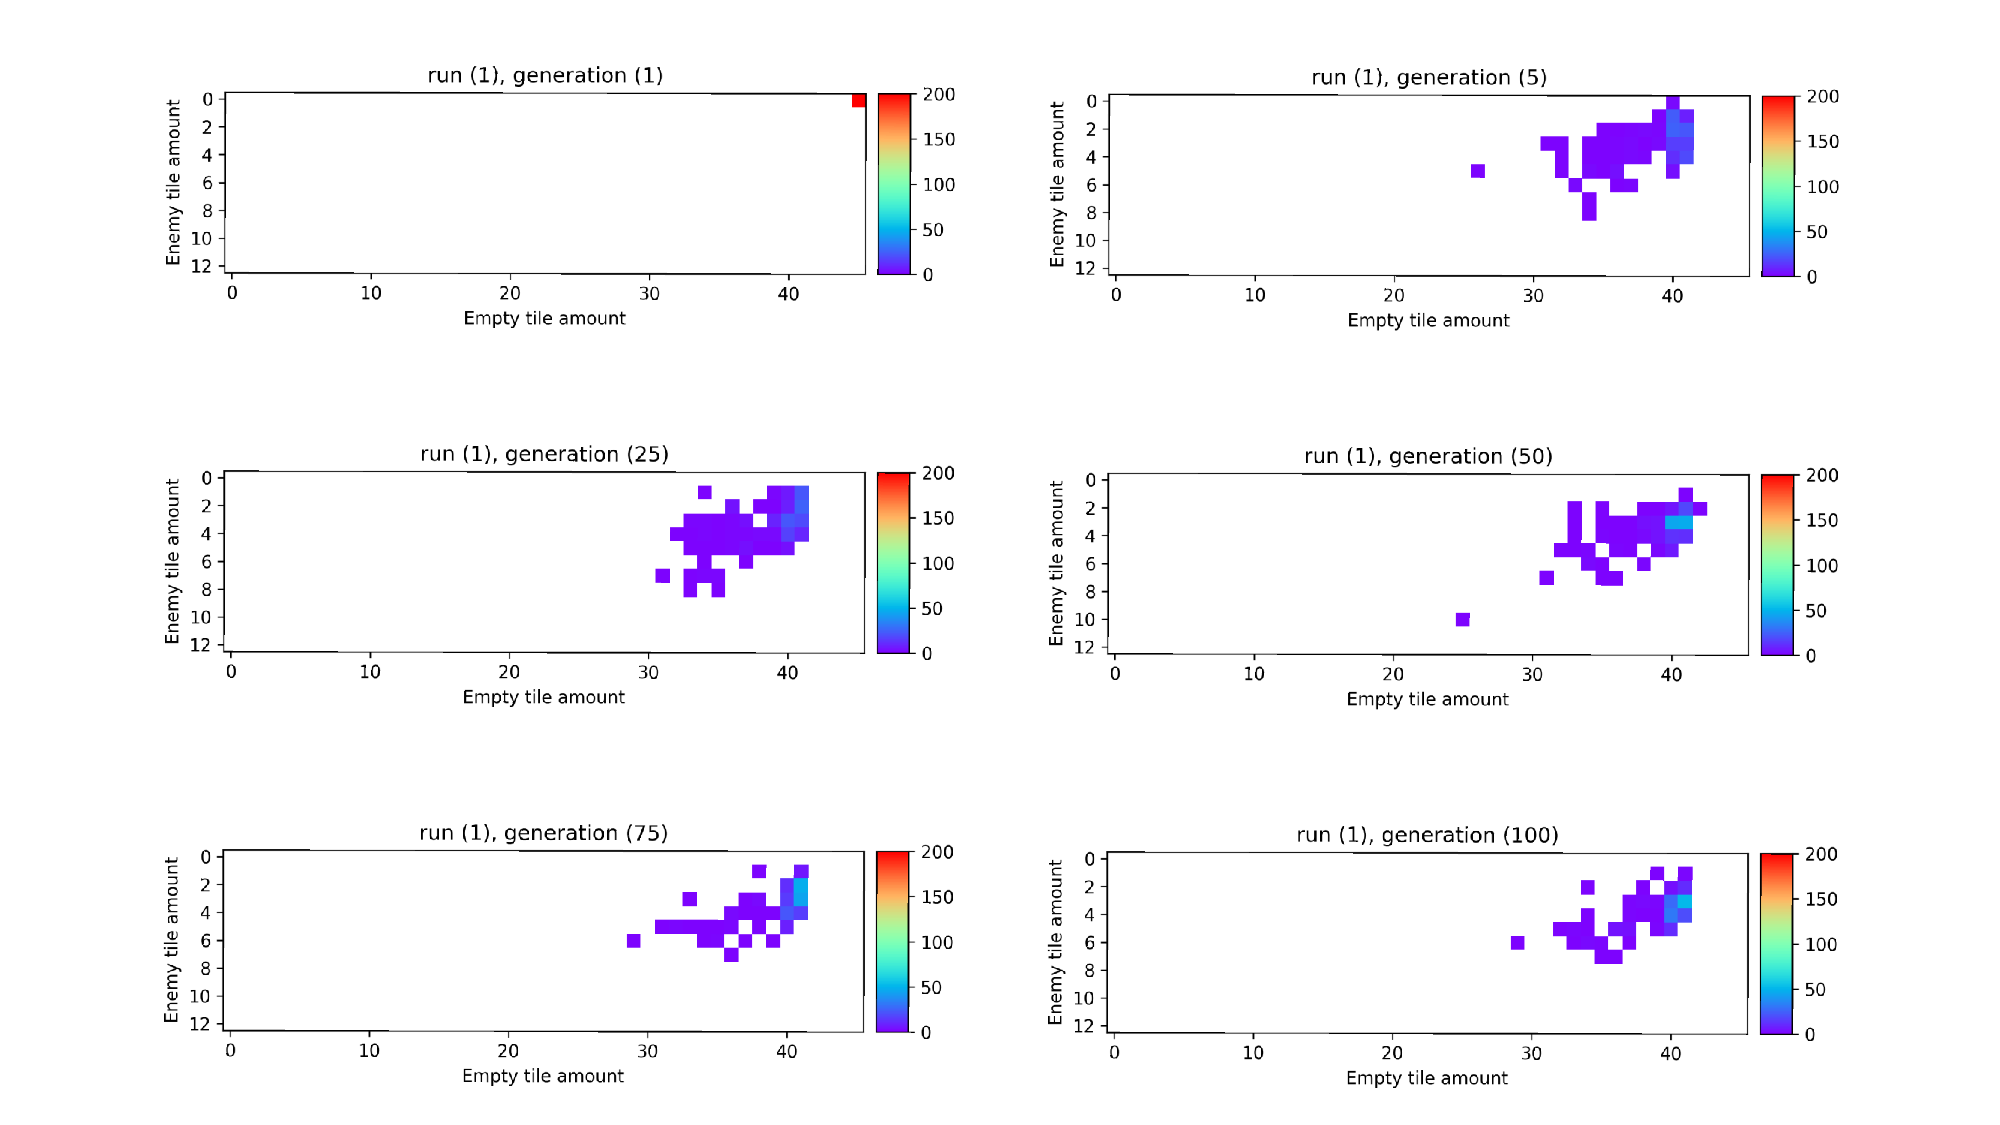
\includegraphics[width=1.0\textwidth]{figures/experiments/experiment-normalized-single-heatmap.pdf}
%     \caption{單一指標型的空磚對敵人磚之數量比例} 
%     \label{fig:experiment-normalized-single-heatmap}
%   \end{center}
% \end{figure}

% \landscapeexperimentpage{
%   \subsection{複合指標型 - 戰鬥通道(狹路驅逐 II)}
%   \label{ssec:experiment-normalized-narrow}

%   \gasettingstable{y1}{Y1}
%     { $5$ & $100$ & $200$ \\ }
%     {
%       阻擋點       & $1.00$ & \\
%       巡邏點       & $0.75$ & \\
%       遊戲物件數量 & $1.75$ & $Limit: [4, 5]$ \\
%     }

%   % \galayoutresults{y1}{Y1}
% }

% \begin{figure}[H]
%   \begin{center}
%     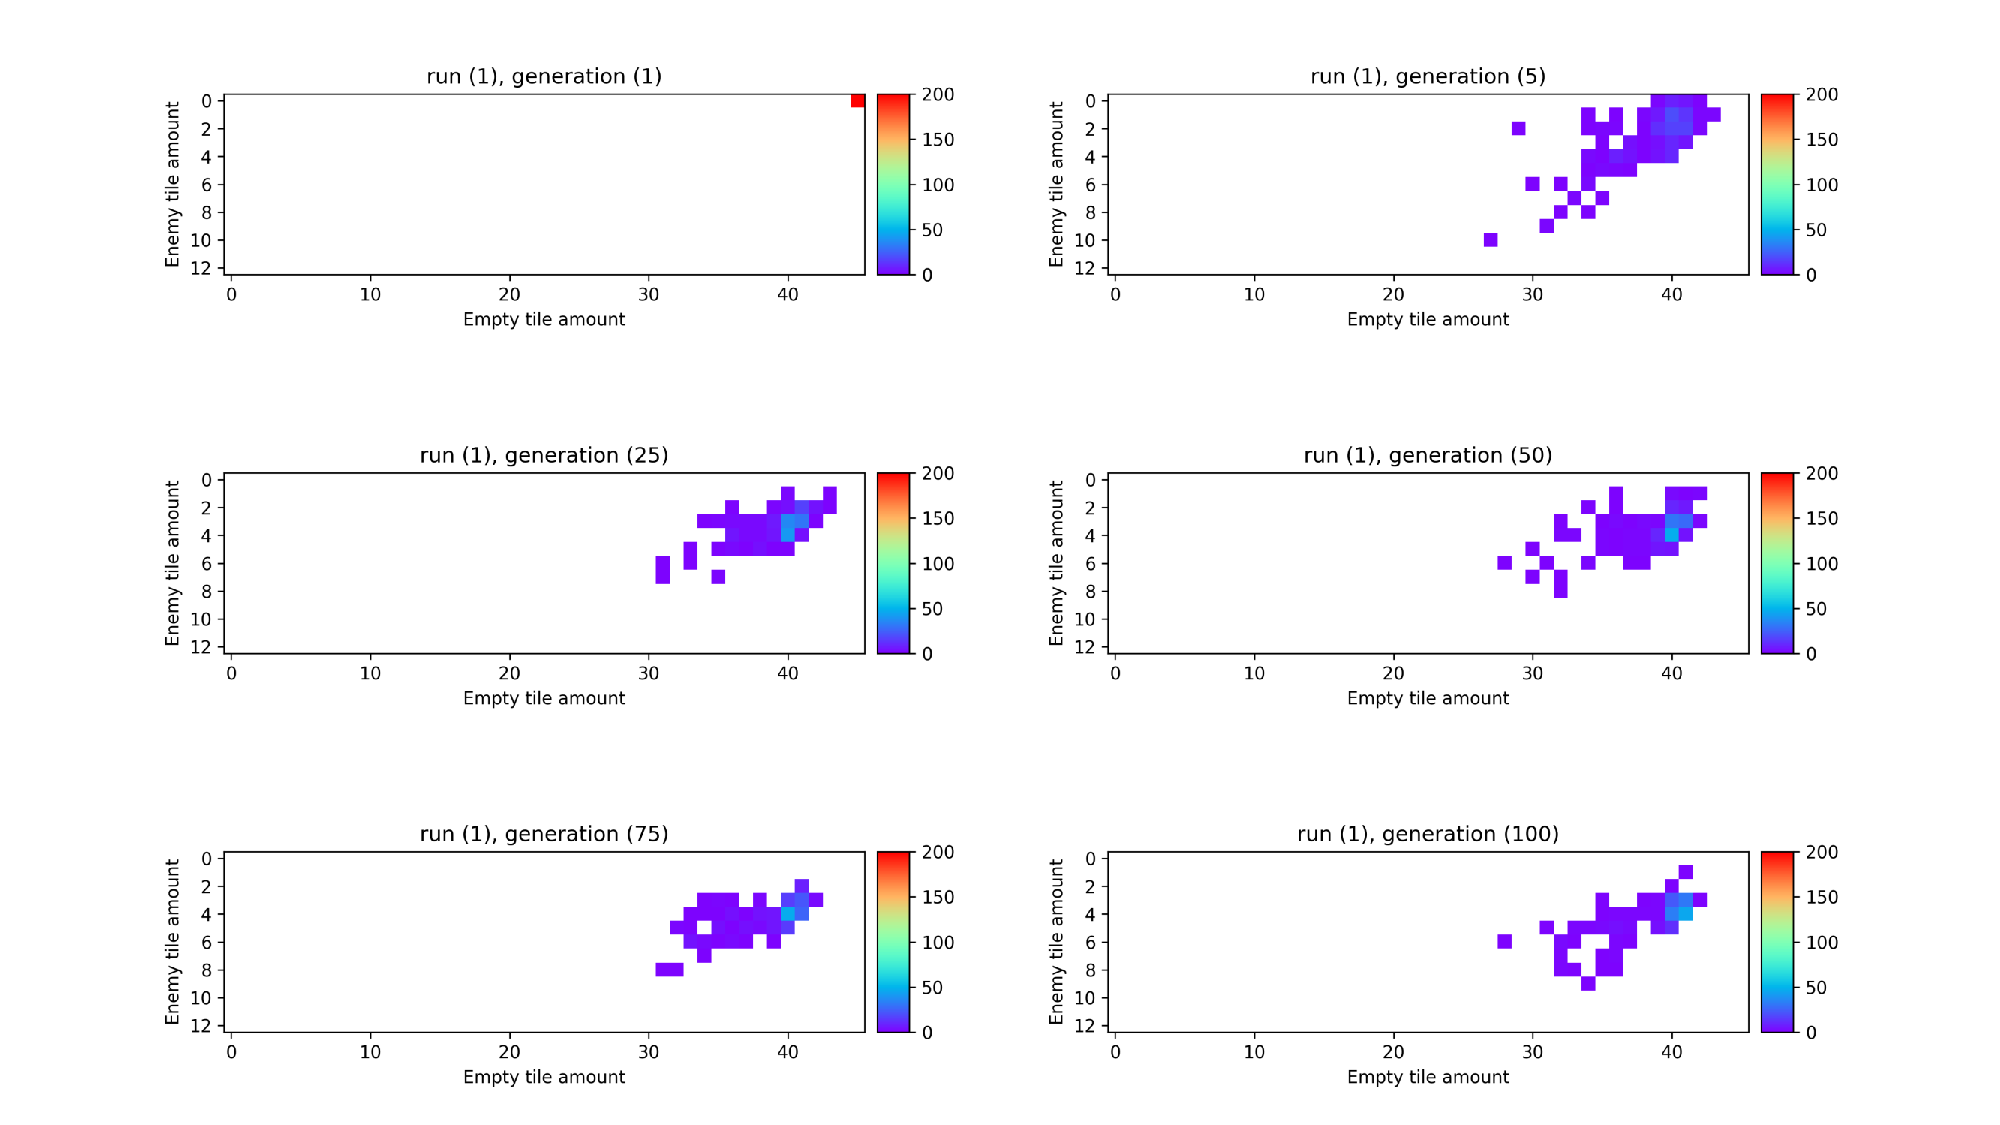
\includegraphics[width=1.0\textwidth]{figures/experiments/experiment-normalized-multi-heatmap.pdf}
%     \caption{複合指標型的空磚對敵人磚之數量比例} 
%     \label{fig:experiment-normalized-multi-heatmap}
%   \end{center}
% \end{figure}


% \section{房型規模之比較}
% \label{sec:experiment-density}

% 房型的大小較有可能直接影響和可行走瓦磚之數量。本階段的實驗中,我們提取第~\ref{sec:experiment-datacollection} 節的資料,將空白、敵人兩種類型的數量關係繪製成熱圖進行觀察。這是因為各項適應性函數在設計時,多以「敵人」與其餘敵人、其它遊戲物件或玩家動線為考量參考,因而推估二者間勢必存在者某些關係。





